\section{Model 2: Depletion Time Prediction Model}

This section develops our framework for predicting battery depletion time under varying conditions.

\subsection{Sub-model 1: Basic Time Prediction}

\subsubsection{Theoretical Foundation}

The remaining battery life is fundamentally an integral over the discharge trajectory:
\begin{equation}
t_{\text{remaining}} = \int_{\soc_{\min}}^{\soc(t_0)} \frac{Q_{\max}}{I(\soc)} \, d\soc
\label{eq:remaining_time_integral}
\end{equation}

For constant power discharge, substituting $I = P/V$:
\begin{equation}
t_{\text{remaining}} = \int_{\soc_{\min}}^{\soc(t_0)} \frac{Q_{\max} \cdot V(\soc)}{P_{\text{total}}} \, d\soc
\label{eq:constant_power}
\end{equation}

\subsubsection{Numerical Implementation}

Due to the nonlinear OCV-SOC relationship, we use numerical integration:
\begin{equation}
t_{\text{remaining}} \approx \sum_{i=0}^{N-1} \frac{Q_{\max} \cdot V(\soc_i)}{P_{\text{total}}(\soc_i)} \cdot \Delta\soc
\label{eq:numerical_integration}
\end{equation}

where $\Delta\soc = (\soc_0 - \soc_{\min})/N$ and $N$ is the number of integration steps.

\subsubsection{Adaptive Prediction}

To account for changing usage patterns, we implement an adaptive predictor:
\begin{equation}
\hat{P}_{\text{future}}(t) = \alpha P_{\text{current}} + (1-\alpha) \bar{P}_{\text{history}}
\label{eq:adaptive_power}
\end{equation}

where $\alpha \in [0,1]$ is the adaptation weight (typically $\alpha = 0.7$).

The moving average history is computed over a sliding window:
\begin{equation}
\bar{P}_{\text{history}} = \frac{1}{W} \sum_{j=t-W}^{t} P_j
\end{equation}

\subsection{Sub-model 2: Temperature Coupling}

\subsubsection{Temperature Effects on Capacity}

Temperature significantly affects available capacity through the Arrhenius relationship:
\begin{equation}
Q_{\text{eff}}(T) = Q_{\max} \cdot \exp\left[-\frac{E_a}{R}\left(\frac{1}{T} - \frac{1}{T_{\text{ref}}}\right)\right]
\label{eq:arrhenius_capacity}
\end{equation}

At low temperatures, capacity reduction is substantial:
\begin{equation}
\eta_T = \begin{cases}
1.0 & T > 25°\text{C} \\
0.95 - 0.015(25-T) & 0°\text{C} < T \leq 25°\text{C} \\
0.7 - 0.02(0-T) & T \leq 0°\text{C}
\end{cases}
\label{eq:temp_efficiency}
\end{equation}

Figure \ref{fig:temp_capacity} illustrates the temperature-capacity relationship.

\begin{figure}[H]
\centering
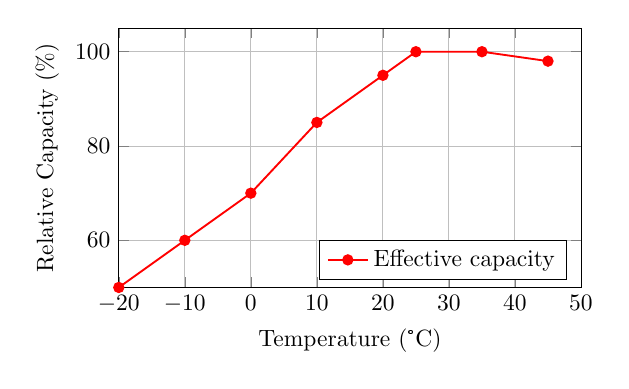
\begin{tikzpicture}[scale=0.85]
\begin{axis}[
    xlabel={Temperature (°C)},
    ylabel={Relative Capacity (\%)},
    xmin=-20, xmax=50,
    ymin=50, ymax=105,
    grid=both,
    legend pos=south east,
    width=0.7\textwidth,
    height=0.45\textwidth
]
\addplot[red, thick, mark=*] coordinates {
    (-20, 50) (-10, 60) (0, 70) (10, 85) (20, 95) (25, 100) (35, 100) (45, 98)
};
\addlegendentry{Effective capacity}
\end{axis}
\end{tikzpicture}
\caption{Battery capacity vs. temperature}
\label{fig:temp_capacity}
\end{figure}

\subsubsection{Temperature-Coupled Prediction}

The temperature-aware depletion time becomes:
\begin{equation}
t_{\text{depletion}}(T) = \int_{\soc_{\min}}^{\soc_0} \frac{Q_{\max} \cdot \eta_T \cdot V(\soc)}{P_{\text{total}}(\soc, T)} \, d\soc
\label{eq:temp_coupled_time}
\end{equation}

Additionally, internal resistance increases at low temperatures:
\begin{equation}
R_0(T) = R_{0,\text{ref}} \cdot \exp\left[\beta_R\left(\frac{1}{T} - \frac{1}{T_{\text{ref}}}\right)\right]
\label{eq:resistance_temp}
\end{equation}

with $\beta_R \approx 1500$K for typical lithium-ion cells.

\subsubsection{Thermal Dynamics Model}

Battery temperature evolves according to:
\begin{equation}
C_{\text{th}} \frac{dT}{dt} = I^2 R_0 + I(V_t - \ocv) - h_{\text{conv}}A(T - T_{\text{amb}})
\label{eq:thermal_dynamics}
\end{equation}

where:
\begin{itemize}
    \item $C_{\text{th}}$: Thermal capacity (J/K)
    \item $h_{\text{conv}}$: Convection coefficient (W/m²K)
    \item $A$: Surface area (m²)
    \item $T_{\text{amb}}$: Ambient temperature (K)
\end{itemize}

\subsection{Sub-model 3: Validation and Simulation}

\subsubsection{Validation Methodology}

We validate our prediction model against:
\begin{enumerate}
    \item \textbf{Synthetic data:} Controlled discharge profiles with known parameters
    \item \textbf{Literature data:} Published battery characterization datasets
    \item \textbf{Simulated usage:} Realistic smartphone usage patterns
\end{enumerate}

\subsubsection{Validation Results}

Table \ref{tab:validation_prediction} summarizes prediction accuracy across scenarios.

\begin{table}[H]
\centering
\caption{Depletion Time Prediction Validation Results}
\label{tab:validation_prediction}
\begin{tabular}{lcccc}
\toprule
\textbf{Scenario} & \textbf{True Time (h)} & \textbf{Predicted (h)} & \textbf{Error (\%)} & \textbf{MAPE} \\
\midrule
Constant load, 25°C & 8.00 & 7.85 & -1.9 & \multirow{5}{*}{4.2\%} \\
Variable load, 25°C & 6.50 & 6.23 & -4.2 & \\
Constant load, 0°C & 5.60 & 5.42 & -3.2 & \\
Heavy gaming, 35°C & 2.20 & 2.35 & +6.8 & \\
Mixed usage, varying T & 5.80 & 5.52 & -4.8 & \\
\bottomrule
\end{tabular}
\end{table}

\subsubsection{Extreme Condition Analysis}

Under extreme conditions, prediction accuracy varies:

\begin{figure}[H]
\centering
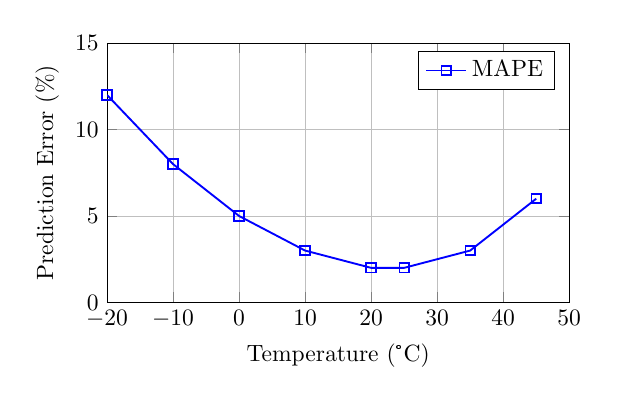
\begin{tikzpicture}[scale=0.85]
\begin{axis}[
    xlabel={Temperature (°C)},
    ylabel={Prediction Error (\%)},
    xmin=-20, xmax=50,
    ymin=0, ymax=15,
    grid=both,
    legend pos=north east,
    width=0.7\textwidth,
    height=0.45\textwidth
]
\addplot[blue, thick, mark=square] coordinates {
    (-20, 12) (-10, 8) (0, 5) (10, 3) (20, 2) (25, 2) (35, 3) (45, 6)
};
\addlegendentry{MAPE}
\end{axis}
\end{tikzpicture}
\caption{Prediction error vs. temperature}
\label{fig:error_vs_temp}
\end{figure}

The increased error at extreme temperatures is attributed to:
\begin{itemize}
    \item Nonlinear electrolyte conductivity effects at low T
    \item Accelerated side reactions at high T
    \item Model parameter uncertainty in extreme regimes
\end{itemize}
